\documentclass[11pt]{article}

% ---------- Packages ----------
\usepackage[margin=1in]{geometry}
\usepackage{amsmath, amssymb}   % math
\usepackage{graphicx}           % \includegraphics
\usepackage{booktabs}           % nicer tables
\usepackage{float}              % [H] placement
\usepackage[font=small, skip=6pt]{caption}
\usepackage{subcaption}         % side-by-side scope captures
\usepackage{xcolor}
\usepackage{listings}        % code blocks, pure TeX (no shell-escape)
\usepackage[hidelinks]{hyperref}

\graphicspath{{pictures/png/}{pictures/photos/}}

% ---------- Code block style (applies to every code block) ----------
% AVR assembly: listings ships no dialect for it, so define one.
\lstdefinelanguage{avrasm}{
  morekeywords={
    add,adc,adiw,sub,subi,sbc,sbci,sbiw,and,andi,or,ori,eor,com,neg,inc,dec,tst,clr,ser,
    mov,movw,ldi,ld,ldd,lds,st,std,sts,push,pop,in,out,lpm,
    cp,cpc,cpi,cpse,breq,brne,brcs,brcc,brsh,brlo,brmi,brpl,brge,brlt,brts,brtc,
    rjmp,jmp,ijmp,rcall,call,icall,ret,reti,nop,sleep,wdr,
    lsl,lsr,rol,ror,asr,swap,sbi,cbi,sbic,sbis,sbrc,sbrs,sbr,cbr,set,clt,
  },
  morekeywords=[2]{.cseg,.dseg,.eseg,.org,.byte,.db,.dw,.equ,.def,.include,.macro,.endmacro},
  alsoletter={.},          % so directives like .cseg tokenize as one word
  morecomment=[l]{;},
  morestring=[b]",
  sensitive=false,
}
\lstdefinestyle{labcode}{
  basicstyle=\ttfamily\small,
  numbers=left, numberstyle=\tiny\color{gray!70}, numbersep=9pt,
  xleftmargin=2.2em, framexleftmargin=2.2em,   % background covers the number gutter
  breaklines=true, breakatwhitespace=true,
  frame=lines, framesep=2mm,
  backgroundcolor=\color{gray!8},
  keywordstyle=\color{blue!65!black}\bfseries,
  keywordstyle=[2]\color{purple!70!black},
  commentstyle=\color{green!40!black},
  stringstyle=\color{orange!85!black},
  showstringspaces=false,
  tabsize=4,
  captionpos=t,
}
\lstset{style=labcode}
\renewcommand{\lstlistingname}{Code}   % caption says "Code 1" instead of "Listing 1"

% ---------- Report info (edit these) ----------
\newcommand{\course}{ECE 3218L}
\newcommand{\labtitle}{Lab 4}
\newcommand{\studentname}{Daniel Xu}
\newcommand{\labdate}{09/30/2026}

% article.cls always typesets title -> author -> date, so the date goes in the
% title block to sit directly under it. \date{} is required; empty means \today.
\title{\labtitle \\[0.3em] \large \labdate}
\author{\studentname \\ \small \course{} \,}
\date{}

% One oscilloscope capture inside a two-column figure.
\newcommand{\scope}[3]{%
  \begin{subfigure}[t]{0.48\textwidth}
    \centering
    \includegraphics[width=\linewidth]{#1}
    \caption{#2}
    \label{#3}
  \end{subfigure}}

\begin{document}
\maketitle

\section{Overview}
Microcontrollers are digital, but many of the signals they must produce are analog. This lab uses the ATmega328P as a signal generator by driving an Analog Devices AD7302 digital-to-analog converter from the PORTD output pins. The programs made sawtooth, triangle, square, trapezoidal, and sine waveforms. The frequency of the waveforms was changed with a delay loop between samples or by skipping points of a lookup table.

\section{Procedure}
Every program writes one sample at a time to the DAC with the same sequence: write the byte to PORTD, pull PC0 low, and return it high, which latches the value into Channel~A. PC1 is cleared once at reset to select Channel A, and PC0 starts high.
Figure~\ref{fig:circuit} shows the circuit on the lab board.

\begin{figure}[H]
  \centering
  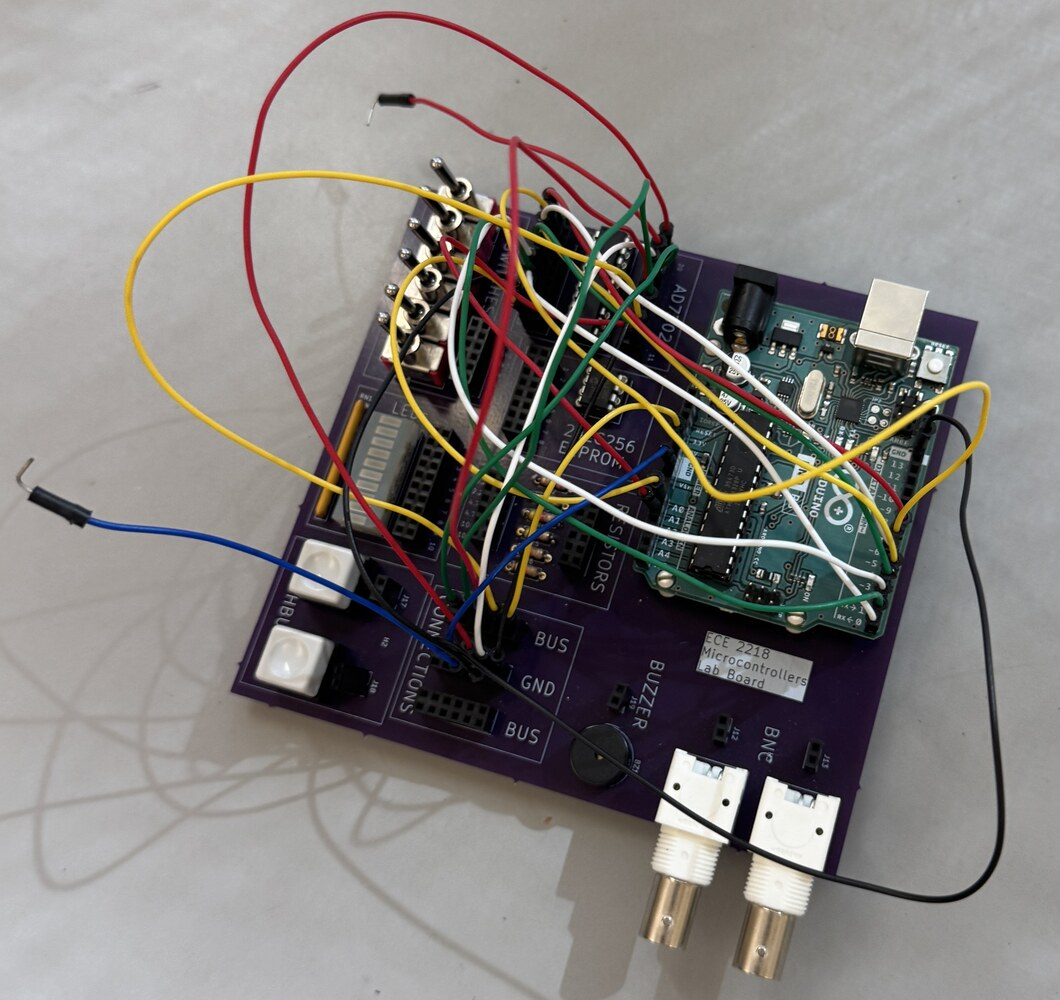
\includegraphics[width=0.6\textwidth]{circuit.jpg}
  \caption{ATmega328P (Arduino Uno) wired to the AD7302 DAC on the lab board.}
  \label{fig:circuit}
\end{figure}

\begin{enumerate}
\item A program was written that loads the series 0x00, 0x01, \ldots, 0xFF, 0x00, \ldots{} into the DAC. 

% TODO: describe the actual sawtooth/triangle/square code once the listings are in.
The sawtooth program increments a register after every sample and wraps from 0xFF to 0x00. The triangle program counts up to 0xFF and then back down to 0x00. The square wave reuses the triangle loop timing but outputs only 0x00 during the ascending half and 0xFF during the descending half, so it has the same frequency as the triangle wave.

\item A program was written to generate a trapezoidal waveform.

% TODO: confirm against the trapezoid listing.
The trapezoid counts up from 0x00 to 0xFF, holds 0xFF for a programmable number of samples, counts back down to 0x00, and holds 0x00 for the same number of samples. The constants TOP\_LENGTH and BOT\_LENGTH set the number of cycles to hold at the top and bottom of the trapezoid. 

\item A program was written to generate a sine wave from a table.

A table was generated with the values from the following equation:
\begin{equation}
  s_k = \operatorname{round}\!\left(127 \sin\frac{\pi k}{32}\right), \qquad k = 0, 1, \ldots, 31,
\end{equation}

This table contains 32 values. The minimum value is at $k=0$, where ${s_k = 0}$. The maximum value is at $k=16$, where $s_k = 127$. By using the 128 as the center of the DAC output, a sine wave can be generated with just these $s_k$ values. The first half of the wave is generated with $128+s_k$ and the second (negative) half is generated with $127-s_k$.

\item A program was written to generate a triangle wave of variable frequency.

By using a delay loop between sample outputs, the frequency of the triangle wave was able to be varied.

\item A program was written to vary the frequency of the sine wave by skipping table points.

By incrementing the table index by more than 1, steps in the table are skipped and the frequency of the sine wave increased.
\end{enumerate}

\begin{table}[H]
  \centering
  \caption{Table of generated sine values from $s_k = \operatorname{round}(127\sin(\pi k/32))$.}
  \label{tab:sine}
  \small
  \begin{tabular}{l*{16}{r}}
    \toprule
    $k$   & 0 & 1 & 2 & 3 & 4 & 5 & 6 & 7 & 8 & 9 & 10 & 11 & 12 & 13 & 14 & 15 \\
    $s_k$ & 0 & 12 & 25 & 37 & 49 & 60 & 71 & 81 & 90 & 98 & 106 & 112 & 117 & 122 & 125 & 126 \\
    \midrule
    $k$   & 16 & 17 & 18 & 19 & 20 & 21 & 22 & 23 & 24 & 25 & 26 & 27 & 28 & 29 & 30 & 31 \\
    $s_k$ & 127 & 126 & 125 & 122 & 117 & 112 & 106 & 98 & 90 & 81 & 71 & 60 & 49 & 37 & 25 & 12 \\
    \bottomrule
  \end{tabular}
\end{table}

\section{Discussion}
\subsection{Output Range}
Writing 0x00 and then 0xFF to PORTD gave a maximum output of $V_\text{max} = 250$~mV. $V_\text{max}$ is set by the reference voltage on REFIN, which this circuit ties to the supply $V_\text{CC}$. A change in the supply or the reference scales the maximum output voltage and the waveforms by the same factor.

\subsection{Measured Waveforms}
All waveforms showed no DC offset on the oscilloscope and spanned $\pm 250$~mV (500~mV peak to peak). This was not expected, as the DAC should output voltages from 0~V to 5~V. Settings on the oscilloscope like AC coupling may have affected the measurements shown, resulting in a peak-to-peak voltage of 500~mV centered at 0V.


Figures~\ref{fig:basic}--\ref{fig:sine} show the oscilloscope images, and Table~\ref{tab:meas} lists the periods and frequencies the oscilloscope measured.

\begin{figure}[tbp]
  \centering
  \scope{newfile8.png}{Sawtooth: 130~$\mu$s, 7.69~kHz.}{fig:saw}\hfill
  \scope{newfile9.png}{Triangle: 286~$\mu$s, 3.50~kHz.}{fig:tri}\\[1em]
  \scope{newfile10.png}{Square: 288~$\mu$s, 3.47~kHz.}{fig:sq}\hfill
  \scope{newfile7.png}{Trapezoid: 515~$\mu$s, 1.94~kHz.}{fig:trap}
  \caption{Sawtooth, triangle, square, and trapezoidal waves.}
  \label{fig:basic}
\end{figure}

\begin{figure}[tbp]
  \centering
  \scope{newfile3.png}{Delay count 10: 1.890~ms, 529~Hz.}{fig:tri10}\hfill
  \scope{newfile4.png}{Delay count 50: 5.760~ms, 174~Hz.}{fig:tri50}
  \caption{Triangle wave with a variable delay loop.}
  \label{fig:trivar}
\end{figure}

\begin{figure}[tbp]
  \centering
  \scope{newfile5.png}{Sine, every point: 40.8~$\mu$s, 24.5~kHz.}{fig:sine1}\hfill
  \scope{newfile6.png}{Sine, every second point: 22.4~$\mu$s, 44.6~kHz.}{fig:sine2}
  \caption{Table-based sine wave.}
  \label{fig:sine}
\end{figure}

\begin{table}[H]
  \centering
  \caption{Measured waveform timing.}
  \label{tab:meas}
  \begin{tabular}{lrrrr}
    \toprule
    Waveform & Period & Frequency \\
    \midrule
    Sawtooth                & 130.0 $\mu$s & 7.692 kHz \\
    Triangle                & 286.0 $\mu$s & 3.497 kHz \\
    Square                  & 288.0 $\mu$s & 3.472 kHz \\
    Trapezoid               & 515.0 $\mu$s & 1.942 kHz \\
    Triangle, delay 10      & 1.890 ms     & 529.1 Hz  \\
    Triangle, delay 50      & 5.760 ms     & 173.6 Hz  \\
    Sine, step 1            & 40.80 $\mu$s & 24.51 kHz \\
    Sine, step 2            & 22.40 $\mu$s & 44.64 kHz \\
    \bottomrule
  \end{tabular}
\end{table}

The waveform shapes match the predictions. At 500~mV peak-to-peak, one DAC step is only about 2~mV, so the waveforms look smooth.

Note that skipping every other point halves the samples per period, but the period drops from 40.8~$\mu$s to 22.4~$\mu$s rather than to 20.4~$\mu$s. The frequency rises by a factor of 1.82 instead of 2, since each run of the skipping loop takes about one cycle longer.

\subsection{Frequency Control with a Delay Loop}
In Program~3, each sample takes $9 + 3N$ cycles, where $N$ is the delay count: 9 cycles for the output and loop control, and $3N - 1$ cycles for the countdown loop plus 1 cycle for the mov that reloads it. One period of the triangle wave has 510 samples, so at 16~MHz the predicted period is
\begin{equation}
  T = \frac{510\,(9 + 3N)}{16 \times 10^{6}\ \text{Hz}}.
\end{equation}
Raising the count from 10 to 50 lengthened the period by
\begin{equation}
  \Delta T_\text{measured} = \frac{5.760~\text{ms} - 1.890~\text{ms}}{50 - 10} = 96.8~\mu\text{s}
\end{equation}
per count, within about 1\% of the predicted $510 \cdot 3 / 16~\text{MHz} = 95.6~\mu$s. So each extra count adds the expected 3 cycles per sample.

\section{Conclusion}
In this lab, the ATmega328P drove an AD7302 DAC through PORTD. The programs generated sawtooth, triangle, square, trapezoidal, and sine waves, all with a span of 500~mV and no DC offset on the oscilloscope. The shape of each waveform matched the prediction. A countdown delay loop between samples lengthened the triangle period by 96.8~$\mu$s per count, within about 1\% of the 95.6~$\mu$s predicted from the cycle count. The other waveforms also matched their cycle counts and expected periods.

\appendix
\section{Full Code}
\label{app:code}

\begin{lstlisting}[language=avrasm,caption={Program 1. Sawtooth, triangle, square, and trapezoidal waves.},label={code:waves}]
.macro DACOUT                   ; DACOUT reg : write reg to DAC channel A
    out  PORTD, @0
    cbi  PORTC, 0
    sbi  PORTC, 0
.endmacro

.equ TOP_LENGTH = 200
.equ BOT_LENGTH = 200

.cseg
.org 0x0000
    rjmp reset

reset:
    ldi  r16, high(RAMEND)
    out  SPH, r16
    ldi  r16, low(RAMEND)
    out  SPL, r16

    sbi  PORTC, 0           ; PC0 = 1
    cbi  PORTC, 1           ; PC1 = 0 -> channel A (done once)
    sbi  DDRC, 0            ; PC0 output (goes out high, no glitch)
    sbi  DDRC, 1            ; PC1 output

    ldi  r16, 0xFF
    out  DDRD, r16          ; PD7-PD0 = data bus outputs
    clr  r17
    rjmp trapezoid

saw:
    DACOUT r17              ; 1 + 2 + 2 = 5
    inc  r17                ; 1
    rjmp saw                ; 2          -> 8 cycles/step

triangle:
tri_up:                         ; 0x00 to 0xFE
    DACOUT r17
    inc  r17
    cpi  r17, 0xFF
    brne tri_up
tri_down:                       ; 0xFF to 0x01
    DACOUT r17
    dec  r17
    nop
    brne tri_down
    rjmp tri_up

square:
    ldi  r18, 0x00          ; low level
    ldi  r19, 0xFF          ; high level
sq_up:
    DACOUT r18
    inc  r17
    cpi  r17, 0xFF
    brne sq_up
sq_down:
    DACOUT r19
    dec  r17
    nop
    brne sq_down
    rjmp sq_up

trapezoid:
    ldi r21, TOP_LENGTH
    ldi r22, BOT_LENGTH
    clr r17
    ; all sections should sum to 9 clock cycles

trap_bot_init:
    mov r20, r22 ; load bottom length

trap_bot:
    DACOUT r17
    nop
    dec r20
    brne trap_bot

trap_up:
    inc r17
    DACOUT r17
    cpi r17, 0xFE
    brne trap_up

    inc r17
    mov r20, r21

trap_top:
    DACOUT r17
    nop
    dec r20
    brne trap_top

trap_down:
    dec r17
    DACOUT r17
    cpi r17, 0x01
    brne trap_down

    dec r17
    rjmp trap_bot_init
\end{lstlisting}

\begin{lstlisting}[language=avrasm,caption={Program 2. Table-based sine wave with a fixed or variable table step.},label={code:sine}]
.macro DACOUT                   ; DACOUT reg : write reg to DAC channel A
    out  PORTD, @0
    cbi  PORTC, 0
    sbi  PORTC, 0
.endmacro

.equ SKIP = 2                   ; table step per sample (1 to 31)

.cseg
.org 0x0000
    rjmp reset

reset:
    ldi  r16, high(RAMEND)
    out  SPH, r16
    ldi  r16, low(RAMEND)
    out  SPL, r16

    sbi  PORTC, 0           ; PC0 = 1
    cbi  PORTC, 1           ; PC1 = 0 -> channel A (done once)
    sbi  DDRC, 0            ; PC0 output (goes out high, no glitch)
    sbi  DDRC, 1            ; PC1 output

    ldi  r16, 0xFF
    out  DDRD, r16          ; PD7-PD0 = data bus outputs
    clr  r17
    rjmp sine_skip

sine:
    ldi  r19, 0x80          ; XOR mask: 0x80 = positive half, 0x7F = negative half
    ldi  r24, 0x00          ; WR low  (PC1 = 0 -> channel A)
    ldi  r25, 0x01          ; WR high (PC1 = 0 -> channel A)

sine_half:
    ldi  ZL, low(sine_table*2)    ; Z -> start of table (byte address)
    ldi  ZH, high(sine_table*2)
    ldi  r18, 32                ; 32 samples per half-cycle

sine_loop:
    lpm  r17, Z+            ; 3  fetch table vlaue, advance pointer
    eor  r17, r19           ; 1  -> 128+T or 127-T
    out  PORTD, r17         ; 1  data onto bus
    out  PORTC, r24         ; 1  WR low
    out  PORTC, r25         ; 1  WR high -> latched
    dec  r18                ; 1
    brne sine_loop          ; 2, 10 cycles/sample

    com  r19                ; swap halves: 0x80 <-> 0x7F
    rjmp sine_half

sine_skip:
        ldi  r19, 0x80          ; XOR mask: positive half
        ldi  r24, 0x00          ; WR low,  channel A
        ldi  r25, 0x01          ; WR high, channel A
        ldi  r22, SKIP          ; load step size
        ldi  ZH, high(sine_table*2)
        ldi  ZL, low(sine_table*2)    ; = 0x00 because the table is aligned

ss_loop:
        lpm  r17, Z             ; 3  fetch table value
        eor  r17, r19           ; 1  -> 128+T or 127-T
        out  PORTD, r17         ; 1
        out  PORTC, r24         ; 1  WR low
        out  PORTC, r25         ; 1  WR high
        add  ZL, r22            ; 1  index += K
        cpi  ZL, 32             ; 1  past end of half-cycle?
        brlo ss_loop            ; 2      -> 11 cycles/sample

        subi ZL, 32             ; wrap index, keeping the remainder
        com  r19                ; switch halves: 0x80 <-> 0x7F
        rjmp ss_loop            ; wrap samples take 14 cycles

.org 0x0200                     ; word 0x200 = byte 0x400 -> low byte 0x00
sine_table:
    .db   0,  12,  25,  37,  49,  60,  71,  81
    .db  90,  98, 106, 112, 117, 122, 125, 126
    .db 127, 126, 125, 122, 117, 112, 106,  98
    .db  90,  81,  71,  60,  49,  37,  25,  12
\end{lstlisting}

\begin{lstlisting}[language=avrasm,caption={Program 3. Triangle wave with variable frequency.},label={code:trivar}]
.equ DELAY = 10                 ; delay count per step (1..255)

.macro DACOUT                   ; DACOUT reg : write reg to DAC channel A
    out  PORTD, @0
    cbi  PORTC, 0
    sbi  PORTC, 0
.endmacro

.equ TOP_LENGTH = 3
.equ BOT_LENGTH = 3

.cseg
.org 0x0000
    rjmp reset

reset:
    ldi  r16, high(RAMEND)
    out  SPH, r16
    ldi  r16, low(RAMEND)
    out  SPL, r16

    sbi  PORTC, 0           ; PC0 = 1
    cbi  PORTC, 1           ; PC1 = 0 -> channel A (done once)
    sbi  DDRC, 0            ; PC0 output (goes out high, no glitch)
    sbi  DDRC, 1            ; PC1 output

    ldi  r16, 0xFF
    out  DDRD, r16          ; PD7 to PD0 = data bus outputs
    clr  r17
    rjmp triangle

triangle:
        ldi  r21, DELAY         ; delay count (change this to change frequency)
        clr  r17

triangle_up:                        ; 0x00 -> 0xFE
        DACOUT r17              ; 5
        mov  r20, r21           ; 1
triangle_d1:
        dec  r20                ; 1
        brne triangle_d1        ; 2 (N iterations = 3N - 1 cycles)
        inc  r17                ; 1
        cpi  r17, 0xFF          ; 1
        brne triangle_up        ; 2 -> 9 + 3N cycles/step

triangle_down:                      ; 0xFF -> 0x01
        DACOUT r17              ; 5
        mov  r20, r21           ; 1
triangle_d2:
        dec  r20                ; 1
        brne triangle_d2        ; 2 (3N - 1 cycles)
        dec  r17                ; 1
        nop                     ; 1  pad to match 'up'
        brne triangle_down      ; 2 -> 9 + 3N cycles/step
        rjmp triangle_up
\end{lstlisting}

\end{document}
